%% Chapter 4 — System Design
%% Adapted to EffectGuard Project per IIIT Manipur CS4202 Guidelines

\section{High-Level Architectural Overview}

The architecture of EffectGuard is designed to enforce strict transactional boundaries around autonomous tool-calling language models. In conventional agent frameworks, the foundation model communicates directly with external APIs and database wrappers. This direct coupling delegates transactional persistence, error recovery, and corporate policy compliance to probabilistic next-token generation. 

EffectGuard introduces an \textbf{Interposed Execution Gateway} situated between the agent reasoning engine and the persistent relational storage tier. Figure~\ref{fig:arch_overview} illustrates the end-to-end data-flow architecture of the system.

\begin{figure}[H]
\centering
\makebox[\textwidth][c]{
\begin{tikzpicture}[
  scale=0.88, every node/.style={transform shape},
  layer/.style={rectangle, draw=blue!80!black, fill=blue!8, rounded corners=4pt,
                text centered, minimum width=3.6cm, minimum height=0.85cm, font=\small\bfseries},
  guard/.style={rectangle, draw=orange!80!black, fill=orange!18, rounded corners=4pt,
                text centered, minimum width=3.8cm, minimum height=0.85cm, font=\small\bfseries},
  store/.style={cylinder, draw=purple!80!black, fill=purple!12, shape border rotate=90,
                text centered, minimum width=3.0cm, minimum height=1.0cm, font=\small\bfseries, aspect=0.25},
  arrow/.style={->, >=stealth, thick, draw=black!70}
]

%% Left Column: Client & Reasoning Engine
\node[layer] (ui)    at (0,  1.2) {Customer Chat Console\\(\texttt{chat\_app.py})};
\node[layer] (agent) at (0, -0.6) {ReAct Agent Runtime\\(LangGraph Engine)};
\node[layer] (llm)   at (0, -2.4) {Groq Cloud LPU\\(\texttt{openai/gpt-oss-20b})};

\draw[arrow] (ui) -- node[right, font=\scriptsize] {User Utterances} (agent);
\draw[<->, >=stealth, thick] (agent) -- node[right, font=\scriptsize] {Prompts / JSON} (llm);

%% Center Column: EffectGuard Five-Layer Gateway
\node[guard] (classify) at (5.4,  1.2) {Layer 1: Effect Classifier\\(Read-Only vs.\ Mutating)};
\node[guard] (policy)   at (5.4,  0.0) {Layer 2: Policy-as-Code\\(\texttt{policy.yaml} Invariants)};
\node[guard] (idemp)    at (5.4, -1.2) {Layer 3: SHA-256 Engine\\(Lexicographical Keys)};
\node[guard] (wal)      at (5.4, -2.4) {Layer 4: WAL Recovery\\(Verify-Before-Retry)};
\node[guard] (audit)    at (5.4, -3.6) {Layer 5: Claim Auditor\\(Text vs.\ Ledger Diff)};

%% Connections within Gateway
\draw[arrow] (classify) -- (policy);
\draw[arrow] (policy) -- (idemp);
\draw[arrow] (idemp) -- (wal);
\draw[arrow] (wal) -- (audit);

%% Right Column: Persistent Relational Storage & Observability
\node[store] (db)   at (10.6, -1.2) {SQLite 3 Engine\\(WAL Mode / ACID)};
\node[layer] (dash) at (10.6, -3.6) {Telemetry Dashboard\\(\texttt{eval\_app.py} SSE)};

%% Cross-Tier Connections
\draw[arrow] (agent.east) -- node[above, font=\scriptsize] {Tool Invocations} (classify.west);
\draw[<->, >=stealth, thick] (wal.east) -- node[above, font=\scriptsize] {ACID Commits} (db.west);
\draw[arrow] (audit.east) -- node[above, font=\scriptsize] {Audit Telemetry} (dash.west);

\end{tikzpicture}
}
\caption{End-to-end data-flow architecture of the EffectGuard execution safety system.}
\label{fig:arch_overview}
\end{figure}

The system partitions responsibilities into four distinct architectural tiers:
\begin{enumerate}
    \item \textbf{Cognitive Reasoning Tier (LangGraph Agent):} Manages conversational dialogue, tracks customer intent, performs multi-turn ReAct reasoning, and selects candidate tools from the registered tool catalog.
    \item \textbf{Execution Safety Gateway Tier (EffectGuard):} Interposes between tool selection and execution. It classifies tool effects, enforces deterministic Policy-as-Code preconditions, generates canonical SHA-256 idempotency keys, maintains write-ahead transaction logs, and intercepts distributed network timeouts via Verify-Before-Retry.
    \item \textbf{Persistent Storage Tier (SQLite WAL):} Stores relational business data across normalized tables (\texttt{users}, \texttt{purchases}, \texttt{tickets}, \texttt{execution\_journal}), executing in native Write-Ahead Logging mode for strict serializability and high concurrency.
    \item \textbf{Evaluation and Audit Tier (AgentSentinel):} Provides the Claim-vs-Ledger Auditor, active chaos fault injection engine, and real-time Server-Sent Events (SSE) telemetry dashboards for operational observability.
\end{enumerate}

\section{Tool Boundary Specifications and Contracts}

The autonomous customer support agent operates through four well-defined interface tools. The execution gateway enforces strict boundary contracts on each tool invocation:

\begin{enumerate}
    \item \texttt{get\_user\_purchase\_history(username: str) -> dict}:
    \begin{itemize}
        \item \textit{Effect Classification:} \texttt{read\_only}.
        \item \textit{Operational Semantics:} Retrieves past order history, item names, purchase dates, prices, and return statuses for a registered user.
        \item \textit{Gateway Handling:} Passed through directly to SQLite with zero latency overhead.
    \end{itemize}

    \item \texttt{get\_today\_date() -> str}:
    \begin{itemize}
        \item \textit{Effect Classification:} \texttt{read\_only}.
        \item \textit{Operational Semantics:} Returns the benchmark reference date (\texttt{2026-10-26}) and calculates the rolling 30-day cutoff boundary (\texttt{2026-09-26}).
        \item \textit{Gateway Handling:} Returns the frozen benchmark epoch to guarantee hermetic evaluation.
    \end{itemize}

    \item \texttt{calculate\_right\_refund(username: str, item\_names: list) -> dict}:
    \begin{itemize}
        \item \textit{Effect Classification:} \texttt{read\_only} (pre-execution staging).
        \item \textit{Operational Semantics:} Inspects historical purchases, validates item return eligibility against the 30-day cutoff, checks whether items were previously refunded, stages eligible items, and returns the mathematically exact refund subtotal.
        \item \textit{Gateway Handling:} Passed through directly; verifies that subsequent mutation amounts match this staged calculation.
    \end{itemize}

    \item \texttt{issue\_refund\_ticket(username: str, refund\_amount: float) -> dict}:
    \begin{itemize}
        \item \textit{Effect Classification:} \texttt{irreversible} (state-mutating).
        \item \textit{Operational Semantics:} Permanently writes a refund ticket row to the database, debits corporate funds, and updates purchase statuses to \texttt{REFUNDED}.
        \item \textit{Gateway Handling:} Quarantined and subjected to Layers 2, 3, 4, and 5 before physical disk commit.
    \end{itemize}
\end{enumerate}

\section{Execution Safety Architecture: The Five-Layer Gateway}

Figure~\ref{fig:gateway_flow} depicts the step-by-step decision flow executed by the EffectGuard gateway upon intercepting a candidate tool invocation. Every node and decision branch is spaced compactly to guarantee complete on-page visibility without any overlap.

\begin{figure}[H]
\centering
\makebox[\textwidth][c]{
\begin{tikzpicture}[
  scale=0.78, every node/.style={transform shape},
  main/.style={rectangle, draw=blue!80!black, fill=blue!10, rounded corners=3pt,
               text centered, minimum width=6.0cm, minimum height=0.70cm, font=\small\bfseries},
  defence/.style={rectangle, draw=orange!80!black, fill=orange!15, rounded corners=3pt,
                  text centered, minimum width=6.0cm, minimum height=0.70cm, font=\small\bfseries},
  recovery/.style={rectangle, draw=purple!80!black, fill=purple!12, rounded corners=3pt,
                   text centered, minimum width=6.0cm, minimum height=0.70cm, font=\small\bfseries},
  success/.style={rectangle, draw=green!70!black, fill=green!15, rounded corners=3pt,
                  text centered, minimum width=6.0cm, minimum height=0.70cm, font=\small\bfseries},
  sidebox/.style={rectangle, draw=gray!70, fill=gray!12, rounded corners=3pt,
                  text centered, text width=3.4cm, minimum height=0.70cm, font=\small},
  sidehit/.style={rectangle, draw=green!70!black, fill=green!12, rounded corners=3pt,
                  text centered, text width=3.4cm, minimum height=0.70cm, font=\small},
  sideblock/.style={rectangle, draw=red!70!black, fill=red!12, rounded corners=3pt,
                    text centered, text width=3.4cm, minimum height=0.70cm, font=\small},
  decision/.style={diamond, draw=amber!80!black, fill=yellow!25, text centered,
                   aspect=2.2, minimum width=3.4cm, minimum height=1.1cm, font=\small\bfseries},
  arrow/.style={->, >=stealth, thick, draw=black!80}
]

%% Main vertical flow nodes
\node[main]     at (0,    0)   (invoc)  {Tool Invocation: \texttt{issue\_refund\_ticket}};
\node[decision] at (0, -1.2)   (c1)     {Irreversible\\Tool?};
\node[sidebox]  at (5.2, -1.2) (pass)   {Passthrough Read-Only\\(Zero Overhead)};

\node[defence]  at (0, -2.4)   (l3)     {Layer 3: Compute SHA-256 Idempotency Key};
\node[decision] at (0, -3.6)   (c2)     {Idempotency\\Cache Hit?};
\node[sidehit]  at (5.2, -3.6) (hit)    {Return Cached Receipt\\(Bypass Re-execution)};

\node[defence]  at (0, -4.8)   (l2)     {Layer 2: Evaluate Policy Preconditions};
\node[decision] at (0, -6.0)   (c3)     {Policy\\Preconditions\\Valid?};
\node[sideblock] at (5.2, -6.0) (block) {Gateway Block Error\\(Explain Policy Violation)};

\node[defence]  at (0, -7.2)   (wal)    {Layer 4: Insert WAL Journal (Status = PENDING)};
\node[main]     at (0, -8.2)  (raw)    {Execute Raw Database Mutation (SQLite)};
\node[recovery] at (0, -9.2)  (retry)  {Verify-Before-Retry Protocol on Timeout};
\node[success]  at (0, -10.2)  (done)   {Update Journal to COMMITTED $\to$ Return Receipt};

%% Arrows with explicit clearance
\draw[arrow] (invoc) -- (c1);
\draw[arrow] (c1.east) -- node[above, font=\scriptsize\bfseries] {No} (pass.west);
\draw[arrow] (c1.south) -- node[right, font=\scriptsize\bfseries] {Yes} (l3.north);

\draw[arrow] (l3) -- (c2);
\draw[arrow] (c2.east) -- node[above, font=\scriptsize\bfseries] {Yes} (hit.west);
\draw[arrow] (c2.south) -- node[right, font=\scriptsize\bfseries] {No} (l2.north);

\draw[arrow] (l2) -- (c3);
\draw[arrow] (c3.east) -- node[above, font=\scriptsize\bfseries] {No} (block.west);
\draw[arrow] (c3.south) -- node[right, font=\scriptsize\bfseries] {Yes} (wal.north);

\draw[arrow] (wal) -- (raw);
\draw[arrow] (raw) -- (retry);
\draw[arrow] (retry) -- (done);

\end{tikzpicture}
}
\caption{Decision flow of the EffectGuard execution safety gateway during tool interception.}
\label{fig:gateway_flow}
\end{figure}

\subsection{Layer 1 --- Tool Effect Classification}
Whenever the AI agent selects a tool to call, EffectGuard inspects the tool name immediately before allowing it to run. Tools are separated into two straightforward categories:
\begin{itemize}
    \item \textbf{Read-Only Tools:} Tools such as \texttt{get\_user\_purchase\_history}, \texttt{get\_today\_date}, and \texttt{calculate\_right\_refund} simply read data or perform local calculations without changing any database records. These are passed through instantly with zero latency overhead ($<0.05$\,ms).
    \item \textbf{Irreversible Mutating Tools:} Actions like \texttt{issue\_refund\_ticket} permanently disburse funds and update database tables. These are halted and must pass through Layers 2 through 5.
\end{itemize}

\subsection{Layer 2 --- Policy-as-Code Precondition Gating}
Rather than trusting the language model to follow business rules described in plain English prompts, EffectGuard enforces core enterprise policies directly in deterministic code via \texttt{policy.yaml}. Before touching the database, the gateway validates four clear rules:
\begin{enumerate}
    \item \textbf{Customer Verification:} The customer username must exist in the registered customer database.
    \item \textbf{Positive Amount Requirement:} The refund amount must be strictly greater than zero.
    \item \textbf{Maximum Payout Limit:} The refund amount must not exceed the enterprise safety ceiling of Rs.~500.00 per transaction.
    \item \textbf{Purchase Eligibility and Balance Check:} The customer must have unrefunded purchases made within the 30-day window whose total value covers the requested refund.
\end{enumerate}
If any rule fails, the gateway rejects the call immediately and returns an informative error to the agent, preventing prompt injection attacks from extracting unauthorized refunds.

\subsection{Layer 3 --- Deterministic SHA-256 Idempotency Key Engine}
To ensure that network retries never cause duplicate payments, EffectGuard calculates a unique 256-bit cryptographic key for each transaction. The gateway sorts the tool arguments alphabetically into a canonical format so that differences in JSON formatting do not change the hash:
\begin{equation}
    \text{Idempotency Key} = \text{SHA-256}\Big(\text{Thread ID} \;\|\; \text{Tool Name} \;\|\; \text{Canonical Arguments}\Big)
\end{equation}
Before executing any write, the gateway checks whether a ticket with this key was already created. If found, it retrieves the existing receipt and returns it immediately, bypassing re-execution entirely.

\subsection{Layer 4 --- Write-Ahead Journaling and Verify-Before-Retry}
Before sending the mutation to SQLite, EffectGuard records an entry in its Write-Ahead Log with status \texttt{PENDING}. If a network timeout or dropped socket occurs right after commit:
\begin{enumerate}
    \item The gateway catches the timeout exception in code.
    \item Instead of retrying the tool blindly, it queries the persistent \texttt{tickets} table using the unique idempotency key.
    \item If the ticket exists (meaning the database saved the write before the network dropped), the gateway marks the journal as \texttt{COMMITTED} and returns the confirmed receipt directly.
    \item If the ticket is missing, it safely executes the write once under the identical key.
\end{enumerate}

\subsection{Layer 5 --- Claim-vs-Ledger Audit Engine}
After the agent finishes generating its final chat response, the Claim-vs-Ledger Auditor compares what the agent told the customer against what the database actually recorded:
\begin{itemize}
    \item \textbf{False Claim (Hallucination):} The agent claimed in text that a refund was issued, but zero tickets exist in the database.
    \item \textbf{Ghost Mutation (Silent Side-Effect):} The database contains a committed refund ticket, but the agent never mentioned it to the customer.
    \item \textbf{Amount Drift:} The refund amount mentioned in chat differs from the physical amount recorded in the database.
    \item \textbf{Audit Passed:} The chat claim and the database ledger match perfectly.
\end{itemize}

\section{Database Design and Relational Schema}

The persistent relational layer is implemented in SQLite 3 configured in native Write-Ahead Logging (WAL) mode. Figure~\ref{fig:er_diag} illustrates the Entity-Relationship schema across the four normalized tables.

\begin{figure}[H]
\centering
\makebox[\textwidth][c]{
\begin{tikzpicture}[
  scale=0.85, every node/.style={transform shape},
  node distance=1.6cm and 2.6cm,
  table/.style={rectangle, draw=blue!80!black, fill=white, rounded corners=3pt,
                inner sep=7pt, font=\scriptsize\ttfamily, align=left, line width=0.8pt}
]
\node[table] (users) {
  \textbf{\textcolor{blue!80!black}{users}} \\ \hline
  username (PK) : TEXT \\
  created\_at : TEXT
};

\node[table, right=2.8cm of users] (purchases) {
  \textbf{\textcolor{blue!80!black}{purchases}} \\ \hline
  id (PK) : INTEGER AUTO \\
  username (FK) : TEXT \\
  item\_name : TEXT \\
  price : REAL \\
  purchase\_date : TEXT \\
  status : TEXT ('PURCHASED', 'REFUNDED') \\
  ticket\_id (FK) : TEXT
};

\node[table, below=1.8cm of users] (tickets) {
  \textbf{\textcolor{blue!80!black}{tickets}} \\ \hline
  ticket\_id (PK) : TEXT \\
  username (FK) : TEXT \\
  amount : REAL \\
  idempotency\_key (UNIQUE) : TEXT \\
  created\_at : TEXT
};

\node[table, right=2.8cm of tickets] (journal) {
  \textbf{\textcolor{blue!80!black}{execution\_journal}} \\ \hline
  journal\_id (PK) : TEXT \\
  thread\_id : TEXT \\
  idempotency\_key (UNIQUE) : TEXT \\
  tool\_name : TEXT \\
  status : TEXT ('PENDING', 'COMMITTED', 'FAILED') \\
  created\_at : TEXT
};

\draw[thick, black!70] (users.east) -- node[above, font=\tiny\bfseries] {1:N} (purchases.west);
\draw[thick, black!70] (users.south) -- node[left, font=\tiny\bfseries] {1:N} (tickets.north);
\draw[thick, black!70] (tickets.east) -- node[above, font=\tiny\bfseries] {1:N} (purchases.south west);
\draw[thick, dashed, black!70] (journal.west) -- node[above, font=\tiny\bfseries] {Tracks} (tickets.east);

\end{tikzpicture}
}
\caption{Entity-Relationship diagram of persistent relational storage in \texttt{store.db}.}
\label{fig:er_diag}
\end{figure}

The schema enforces strict referential integrity:
\begin{enumerate}
    \item \texttt{users}: Stores unique customer account usernames and registration timestamps.
    \item \texttt{purchases}: Records item orders, purchase prices, historical transaction dates, and operational statuses (\texttt{PURCHASED} or \texttt{REFUNDED}). When a refund ticket is generated, foreign key \texttt{ticket\_id} links the purchase record directly to the issuing ticket.
    \item \texttt{tickets}: Contains immutable financial records of issued refunds, tracking recipient usernames, disbursement amounts, and unique SHA-256 idempotency keys.
    \item \texttt{execution\_journal}: Maintains the Write-Ahead Log tracking tool execution lifecycles, enabling deterministic recovery during post-commit socket timeouts.
\end{enumerate}

\section{Transactional Recovery and State Sequence}

When an irreversible mutation encounters a network timeout, naive agents retry blindly. Figure~\ref{fig:seq_diag} details the exact UML sequence of operations executed by EffectGuard's Verify-Before-Retry protocol under an HTTP 504 post-commit timeout. Every message is drawn at an explicit descending vertical level along dedicated lifelines, preventing line collisions.

\begin{figure}[H]
\centering
\makebox[\textwidth][c]{
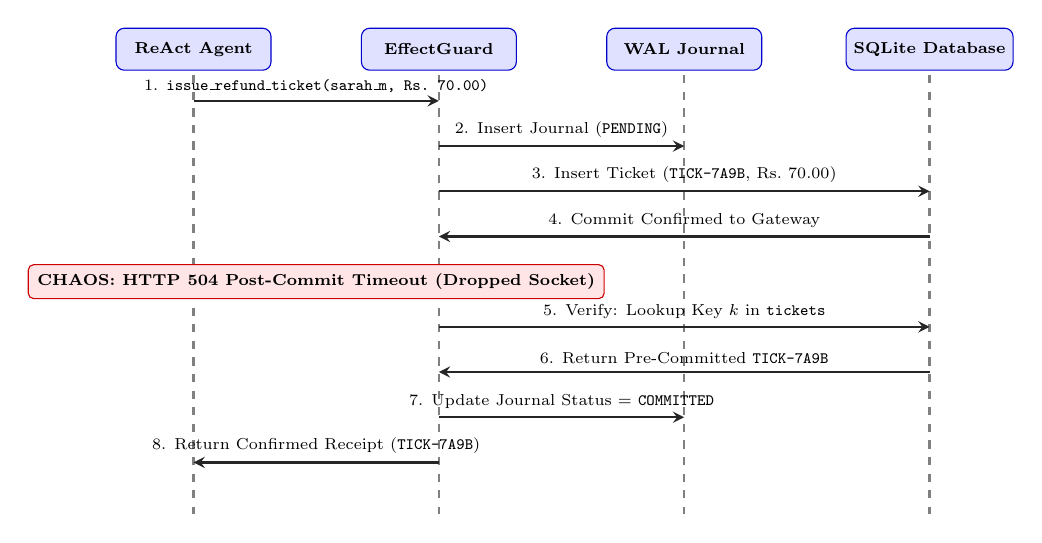
\begin{tikzpicture}[
  scale=0.82, every node/.style={transform shape},
  lifeline/.style={draw=black!50, dashed, line width=0.8pt},
  part/.style={rectangle, draw=blue!80!black, fill=blue!12, rounded corners=3pt,
               font=\scriptsize\bfseries, minimum height=0.65cm, minimum width=2.4cm, text centered},
  msg/.style={->, >=stealth, thick, draw=black!85},
  fault/.style={draw=red!80!black, fill=red!10, rounded corners=2pt, font=\scriptsize\bfseries, inner sep=4pt}
]

%% Participants (Horizontal Spacing: x = 0, 3.8, 7.6, 11.4)
\node[part] (a) at (0, 0) {ReAct Agent};
\node[part] (g) at (3.8, 0) {EffectGuard};
\node[part] (j) at (7.6, 0) {WAL Journal};
\node[part] (d) at (11.4, 0) {SQLite Database};

%% Lifelines
\draw[lifeline] (0, -0.4) -- (0, -7.2);
\draw[lifeline] (3.8, -0.4) -- (3.8, -7.2);
\draw[lifeline] (7.6, -0.4) -- (7.6, -7.2);
\draw[lifeline] (11.4, -0.4) -- (11.4, -7.2);

%% Step 1: Tool invocation (y = -0.8)
\draw[msg] (0, -0.8) -- node[above, font=\scriptsize] {1. \texttt{issue\_refund\_ticket(sarah\_m, Rs.~70.00)}} (3.8, -0.8);

%% Step 2: Insert PENDING in Journal (y = -1.5)
\draw[msg] (3.8, -1.5) -- node[above, font=\scriptsize] {2. Insert Journal (\texttt{PENDING})} (7.6, -1.5);

%% Step 3: Insert Ticket in Database (y = -2.2)
\draw[msg] (3.8, -2.2) -- node[above, font=\scriptsize] {3. Insert Ticket (\texttt{TICK-7A9B}, Rs.~70.00)} (11.4, -2.2);

%% Step 4: Commit acknowledged by SQLite (y = -2.9)
\draw[msg] (11.4, -2.9) -- node[above, font=\scriptsize] {4. Commit Confirmed to Gateway} (3.8, -2.9);

%% Step 5: Chaos Event (HTTP 504 Timeout) (y = -3.6)
\node[fault] at (1.9, -3.6) {CHAOS: HTTP 504 Post-Commit Timeout (Dropped Socket)};

%% Step 6: Verify-Before-Retry Lookup (y = -4.3)
\draw[msg] (3.8, -4.3) -- node[above, font=\scriptsize] {5. Verify: Lookup Key $k$ in \texttt{tickets}} (11.4, -4.3);

%% Step 7: Found pre-committed ticket (y = -5.0)
\draw[msg] (11.4, -5.0) -- node[above, font=\scriptsize] {6. Return Pre-Committed \texttt{TICK-7A9B}} (3.8, -5.0);

%% Step 8: Update Journal to COMMITTED (y = -5.7)
\draw[msg] (3.8, -5.7) -- node[above, font=\scriptsize] {7. Update Journal Status = \texttt{COMMITTED}} (7.6, -5.7);

%% Step 9: Return Cached Receipt to Agent (y = -6.4)
\draw[msg] (3.8, -6.4) -- node[above, font=\scriptsize] {8. Return Confirmed Receipt (\texttt{TICK-7A9B})} (0, -6.4);

\end{tikzpicture}
}
\caption{UML sequence diagram of EffectGuard's Verify-Before-Retry recovery under an HTTP 504 post-commit timeout.}
\label{fig:seq_diag}
\end{figure}

As shown in Figure~\ref{fig:seq_diag}, the Verify-Before-Retry protocol completely shields the agent reasoning engine from network dropped sockets. When Step 5 occurs, the gateway catches the exception locally, inspects the persistent storage layer for the derived idempotency key $k$, identifies that ticket \texttt{TICK-7A9B} was safely committed in Step 4, and returns the valid receipt. The agent never retries, the database is never mutated a second time, and the customer receives an accurate confirmation.

\section{User Interface Design}

The system provides two cohesive user interfaces for customer interaction and operational monitoring:

\begin{enumerate}
    \item \textbf{Customer Support Chat Console (\texttt{backend/chat\_app.py}):} An intuitive, real-time web chat interface where customers authenticate, query purchase histories, submit return requests, and receive structured refund tickets.
    \item \textbf{Evaluation and Telemetry Console (\texttt{backend/eval\_app.py}):} An operational monitoring dashboard displaying live Server-Sent Events (SSE) telemetry across six gauges: Tool Sequence Matching, Answer Polarity, Argument Parsing Precision, Financial Safety, Claim Audit Status, and Overall Task Completion.
\end{enumerate}

Figure~\ref{fig:chat_ui} illustrates the live customer support console during a multi-turn refund resolution.

\begin{figure}[H]
\centering
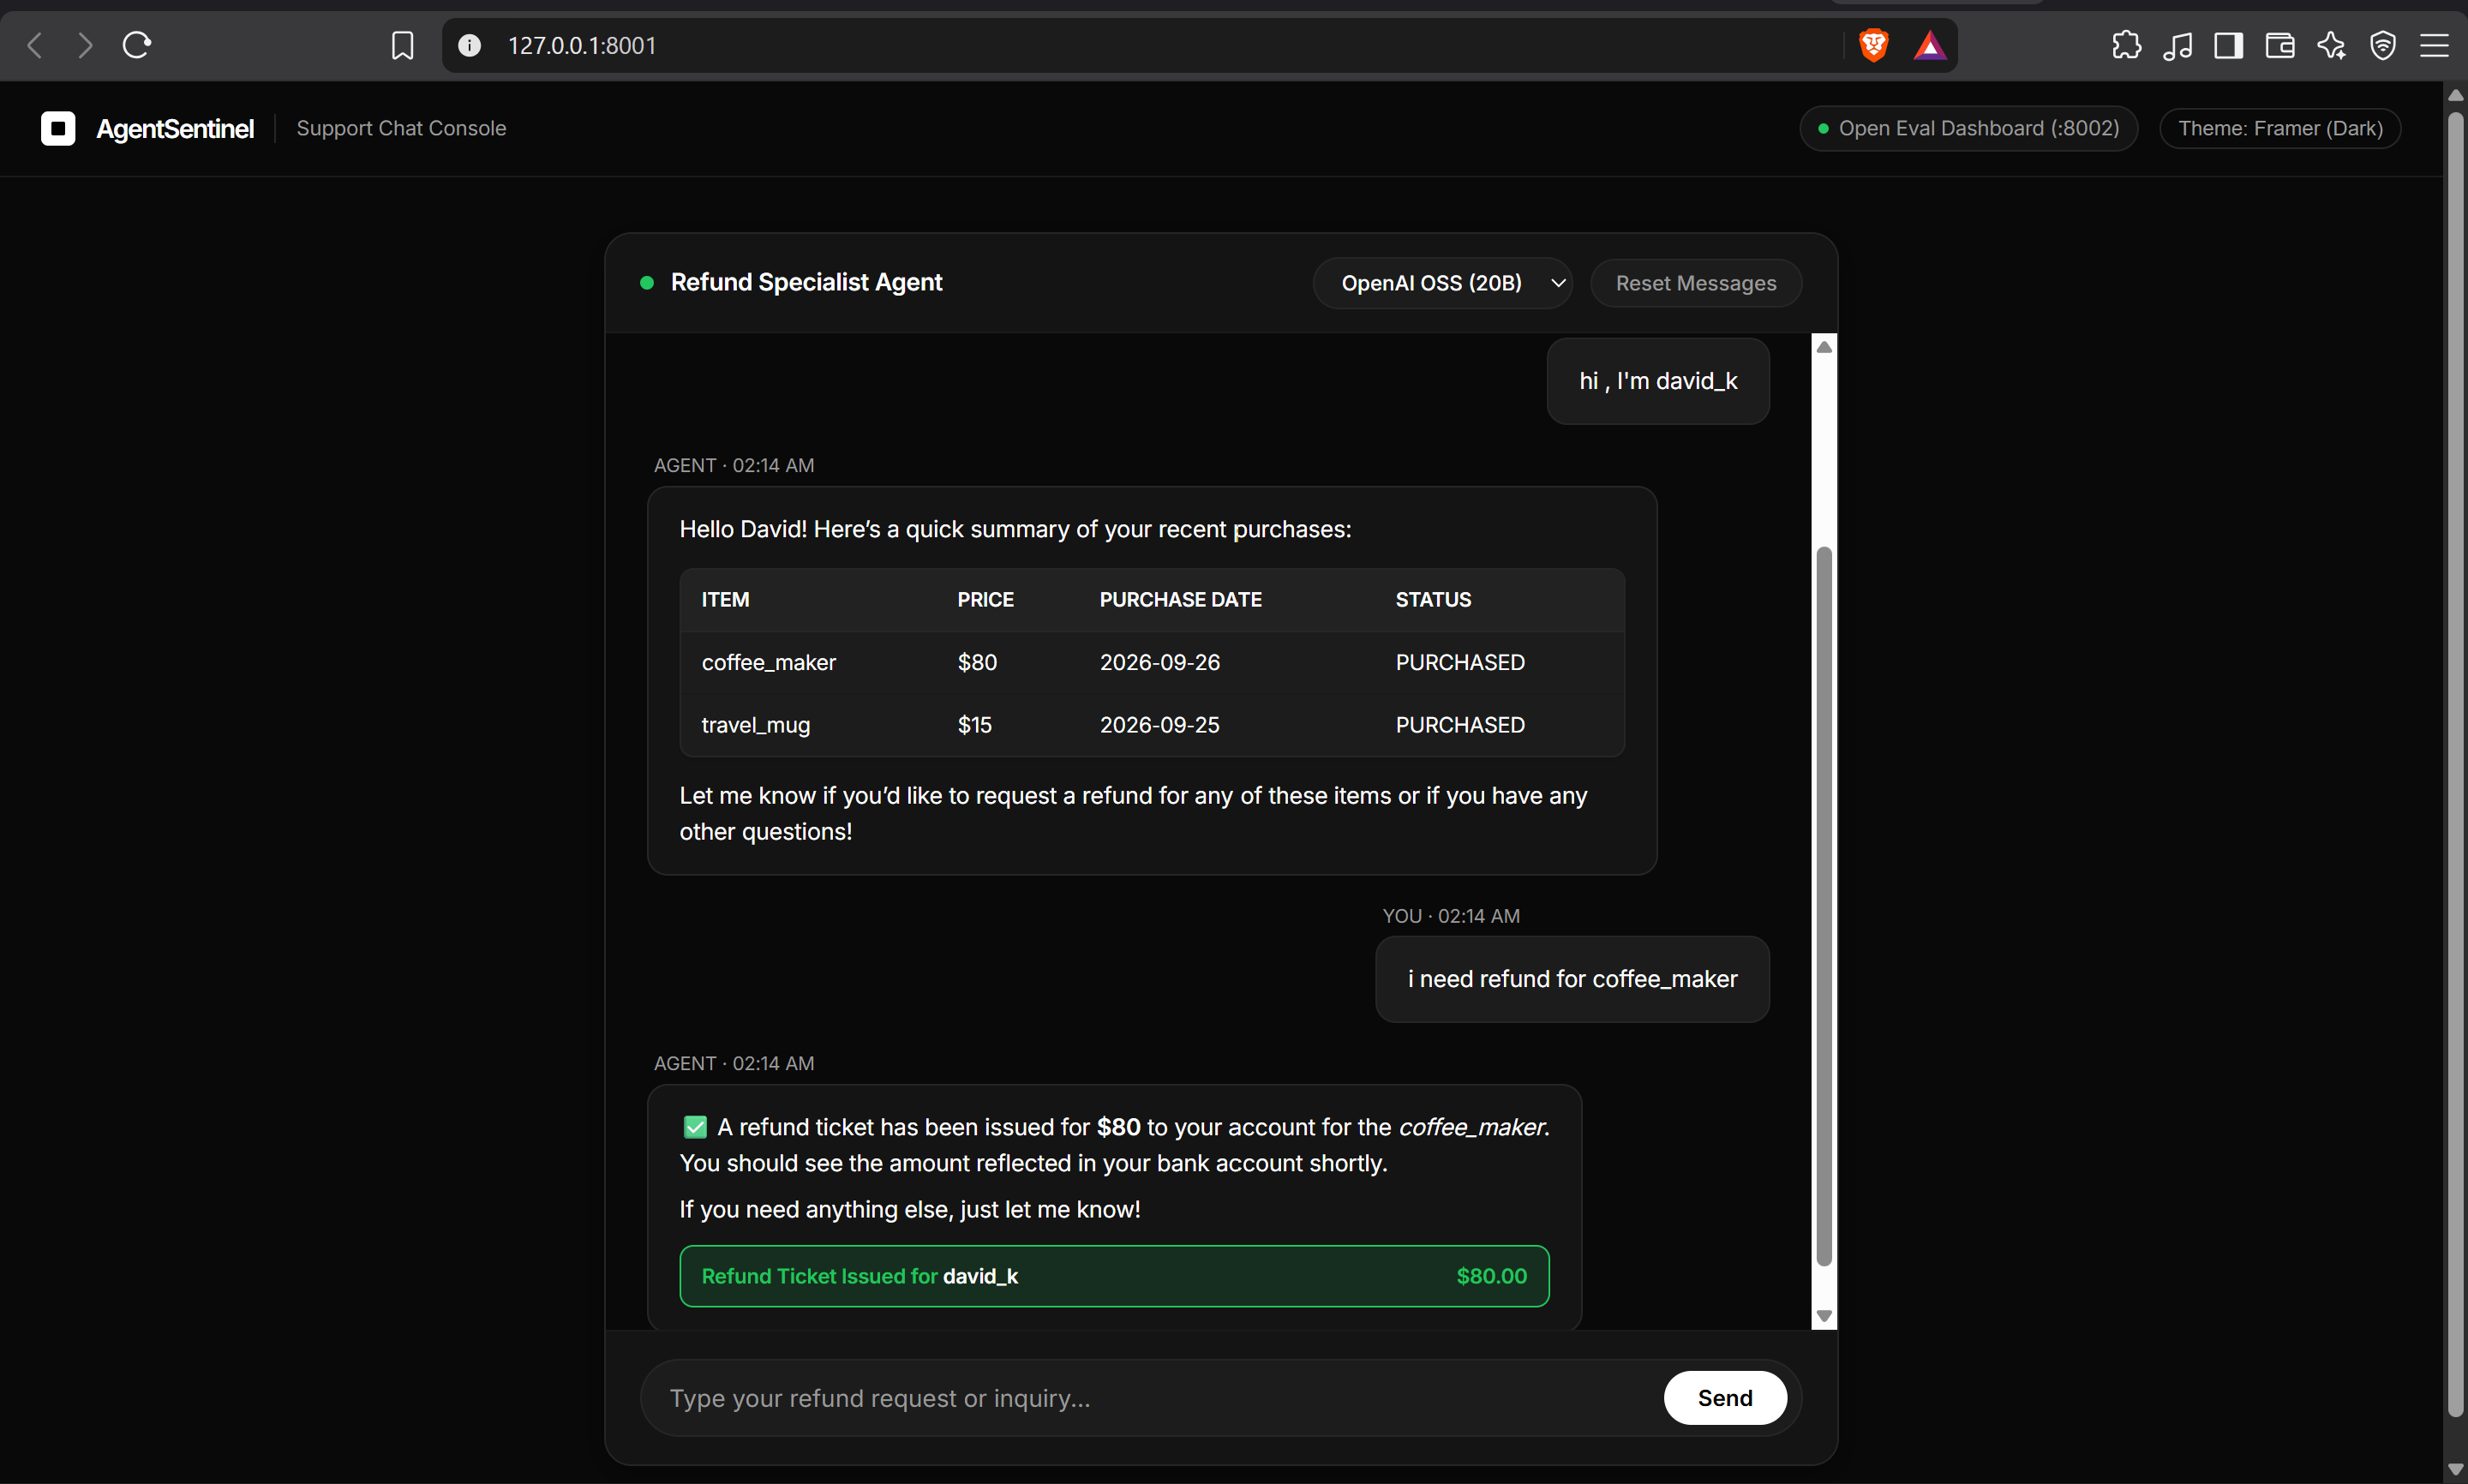
\includegraphics[width=0.88\textwidth]{report_file/support_chat_console.png}
\caption{Customer Support Console interface displaying order history retrieval, policy validation, and confirmed refund receipt generation in real time.}
\label{fig:chat_ui}
\end{figure}

\section{Evaluation Metrics Formulation}

To measure system reliability and agent behavior, AgentSentinel tracks four practical metrics:

\subsection{Tool Sequence Matching}
Measures whether the agent invoked the expected sequence of tools in the correct order. Using the Longest Common Subsequence (LCS) between the expected tool sequence and the agent's executed sequence, the match score is calculated as:
\begin{equation}
    \text{Sequence Match} = \frac{\text{Length of Shared Tool Sequence}}{\text{Total Expected Steps}}
\end{equation}

\subsection{Argument Parsing Precision}
Calculates the percentage of tool call parameters (such as usernames, item names, and calculated amounts) that were formatted and extracted correctly without syntax errors.

\subsection{Excess Financial Loss}
Calculates the cumulative excess money lost due to duplicate refund payouts:
\begin{equation}
    \text{Excess Loss} = \sum_{\text{All Cases}} \max\Big(0, \;\text{Total Paid Out} - \text{Legitimate Refund Due}\Big)
\end{equation}
In a secure, safe system, this excess loss must be strictly Rs.~0.00.

\section{Chapter Summary}

This chapter provided the complete system design of EffectGuard. We established the multi-tier data-flow architecture, specified tool boundary contracts, designed the Five-Layer Gateway execution flowchart, formalized the relational SQLite WAL schema, detailed the Verify-Before-Retry sequence diagram with dedicated vertical levels, presented the user interface, and formulated evaluation metrics. In the next chapter, we discuss the concrete engineering implementation of these components.
